\documentclass[french, 12pt]{article}

\usepackage[T1]{fontenc}
\usepackage[utf8]{inputenc}
\usepackage[french]{babel}

\usepackage{listings}
\usepackage{amsmath}
\usepackage{amssymb}
\usepackage{amsthm}
\usepackage{hyperref}
\usepackage{graphicx}


\title{Rapport Projet Informatique du Métro}
\author{
  Bouarah Romain \and
  Langdorph Matthieu \and
  Ketels Lucas \and
  Souffan Nathan
}


\begin{document}

\maketitle
\begin{abstract}
  Dans le cadre du Projet Informatique du 4ème semestre, voici le projet Métro.
  Ce programme permet de donner le trajet le plus court lors d'un déplacement sur un réseau de métro, représenté par un graphe.
  Ce programme a été développé en Java.
\end{abstract}



\newpage
\tableofcontents



\newpage
\part{Guide d'utilisation du programme}
Voici des indications pour utiliser notre programme "metro". Nous l'avons conçu avec Maven, JUnit et Java.

\section{Installation}
Avant d'installer le programme, il faut vérifier bien avoir Java JDK, Maven et JUnit d'installer sur son ordinateur. Sinon les installer. Il faut également vérifier que les versions sont suffisament à jour, version au moins 8.0 pour Java, au moins 3.6 pour Maven, et au moins 4.11 pour JUnit.
Vous pouvez alors cloner le projet depuis master dans les fichiers de votre ordinateur.
Vous êtes alors prêt pour utiliser "metro".

\section{Utilisation}
Une fois la partie installation effectuée, vous pouvez compiler et exécuter "metro".
Se placer dans le répertoire adapté et se positionner sur master(par défaut).
Pour compiler le projet dans son intégralité, il faut utiliser la commande "make".
Il y a la possibilité de compiler juste datamodel ou le webserver, en faisant suivre leur nom après "make".
On peut compiler les tests avec "make test".
"make clean" supprime tous les fichiers produits pendant la compilation.

Pour exécuter le programme : on peut soit avoir une version minimale sur le terminal avec la commande "make run\_terminal". Sinon on peut avoir la version site Web en utilisant la commande "make run".

Nous allons donc voir comment utiliser le webserver "metro" dans la section suivante.

Nous avons également l'option d'afficher le graphe du réseau d'une ville en utilisant la commande "make export\_to\_dot ARGS="NomDeLaVille" ". Notons que les réseaux de métro des villes de Lille, Lyon, Marseille, Rennes, Toulouse, Paris, et des aéroports de Charles de gaulle et Orly.

\section{Exemple d'exécution}
Nous compilons donc avec la commande "make".
Nous lançons ensuite l'exécution avec "make run".
Apparaît alors un lien :

\begin{lstlisting}
[main] INFO io.javalin.Javalin - Listening on 
http://localhost:8080/
\end{lstlisting}

Il faut alors copier le lien dans un navigateur web pour accéder au webserver de "metro". Cette page ci-dessous s'affiche et on sélectionne alors la ville de notre choix parmi celles possibles. On prend Paris dans cet exemple.

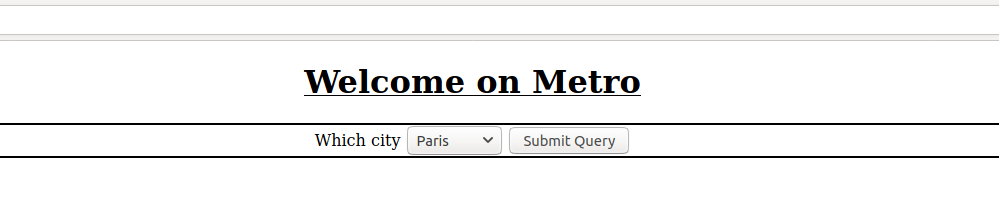
\includegraphics[width=12cm]{images/index.png}

Nous pouvons alors rechercher un itinéraire. Ici de Wagram à Ourcq(Re-marquons qu'il y a autocomplétion de nos stations quand on les recherche). Trois options s'offrent à nous : utiliser Dijkstra(Shortest) pour trouver le plus court chemin, l'algorithme de Floyd ou l'algorithme de Bouarah pour trouver le plus court chemin avec un plafond de nombre de correspondances.

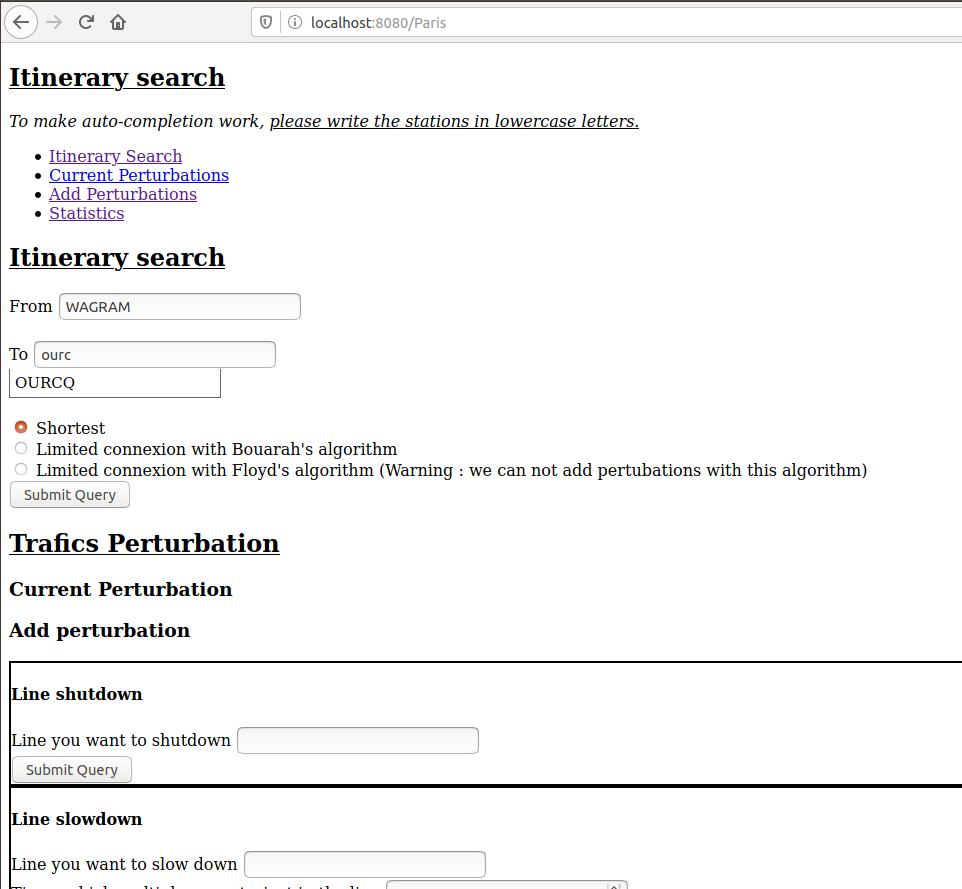
\includegraphics[height=8cm]{images/researchwithoutpert.png}

Nous faisons ici une recherche avec Shortest. S'affichent alors plusieurs itinéraires dans l'ordre croissant en fonction des temps de trajets.

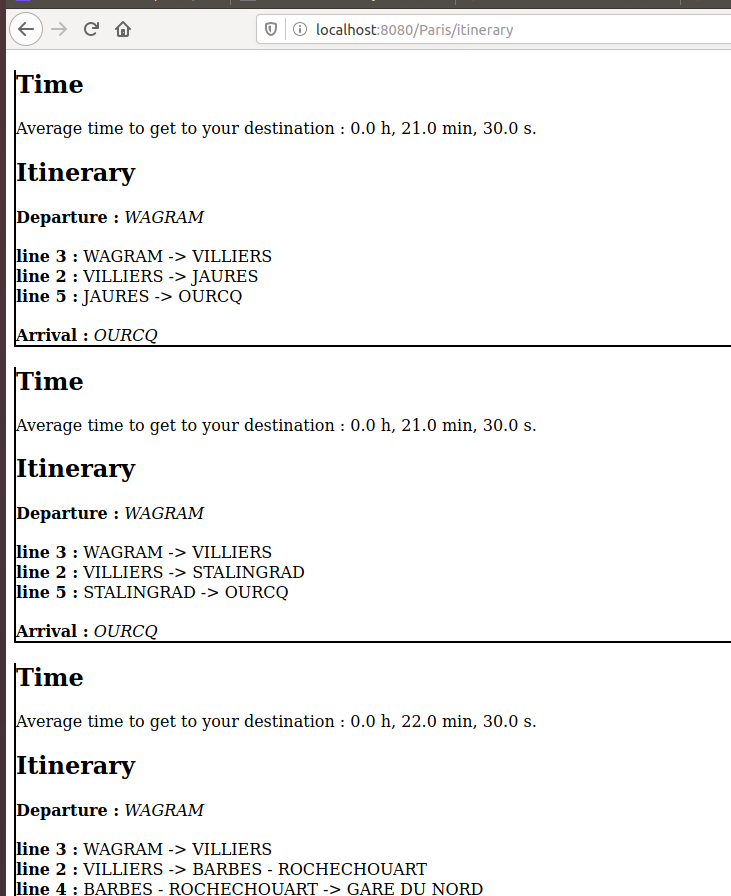
\includegraphics[height=8cm]{images/resultwithoutperturb.png}

Retournons à la page d'avant, on remarque la possibilité d'ajouter des perturbations de trafics. On peut arrêter ou ralentir une ligne ou une partie d'une ligne, fermer une station, fermer une ligne dans une station. Notre itinéraire précédent nous faisais passer par la ligne 2. Fermons donc la ligne 2 puis effectuons la même recherche de trajet entre Wagram et Ourcq.

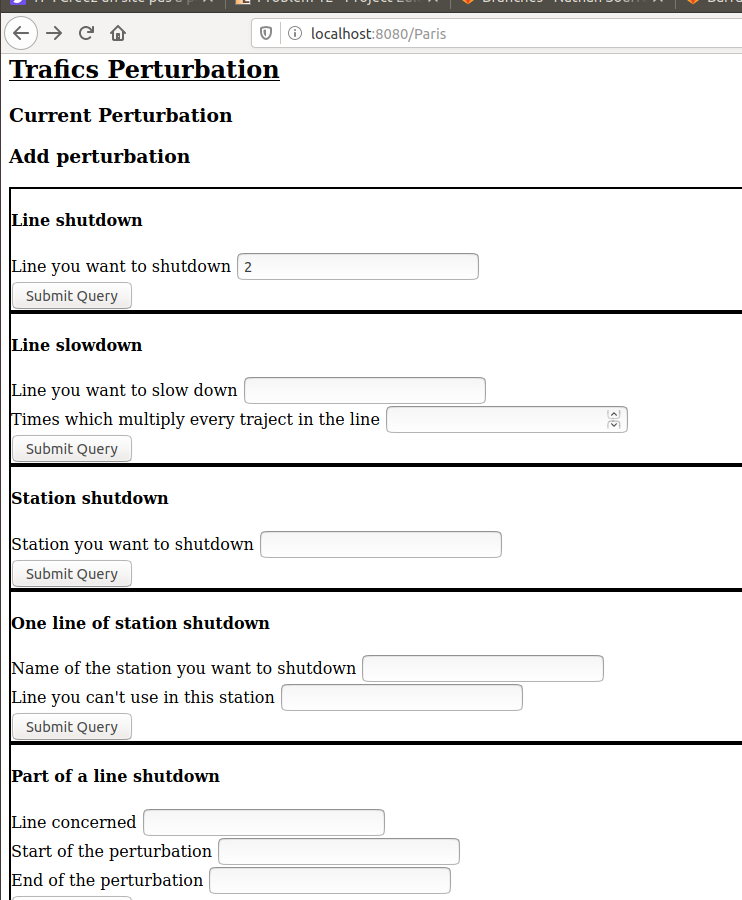
\includegraphics[height=4cm]{images/addpert.png}
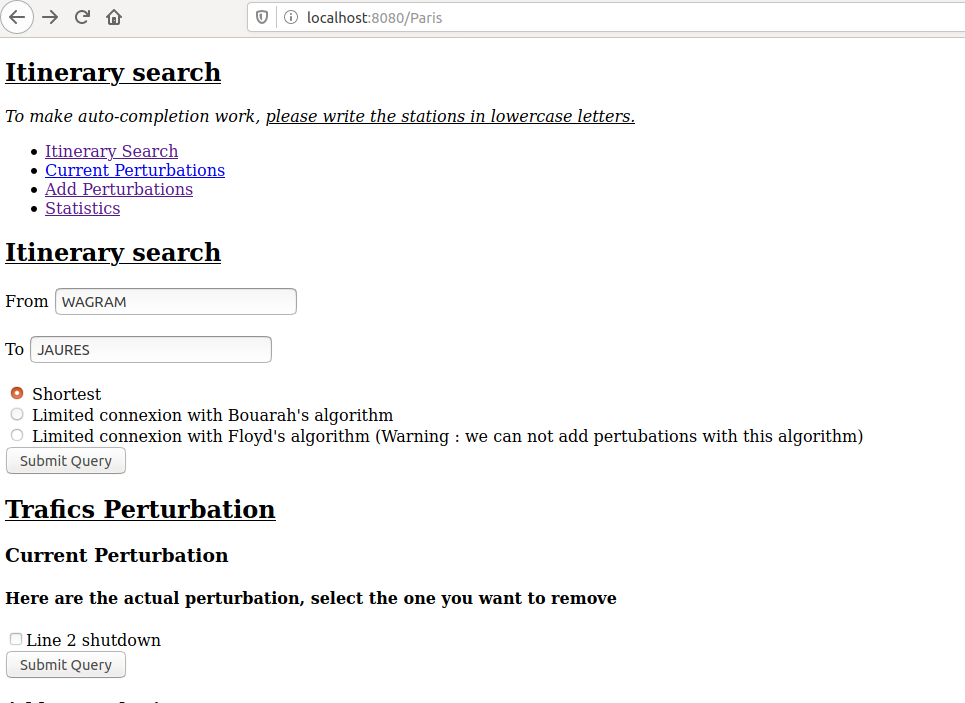
\includegraphics[height=6cm]{images/itiwithpert.png}

On peut à présent voir le trajet le plus court sachant que la ligne 2 est fermée.

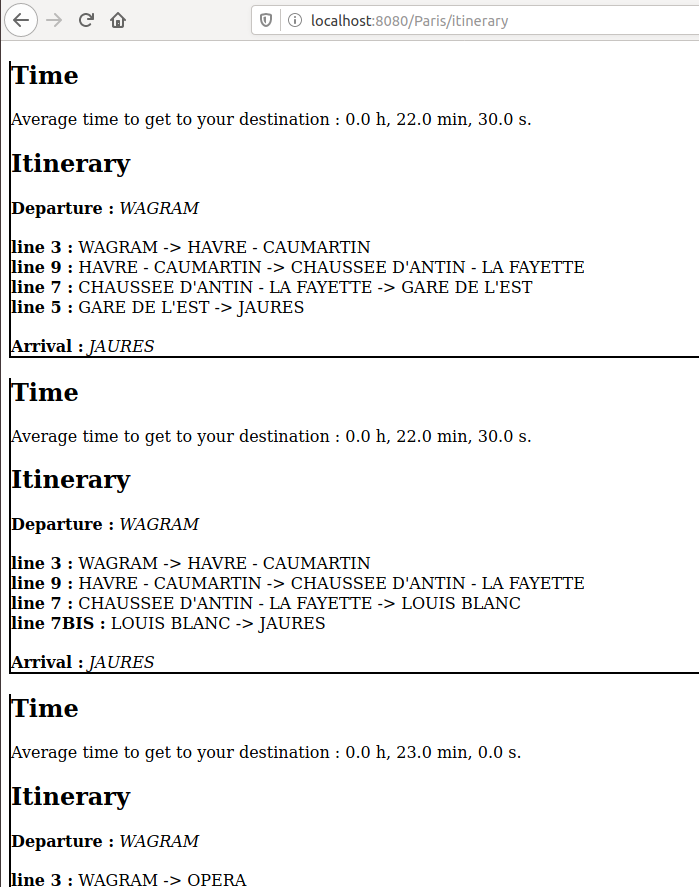
\includegraphics[height=8cm]{images/resultswithpert.png}

Retournons maintenant à la page d'avant, on peut voir tout en haut un menu avec une option "Statistics" qui est alors un lien vers une page affichant les statistiques du réseau de métro de la ville sélectionnée au préalable.
Voici l'affichage de cette page :

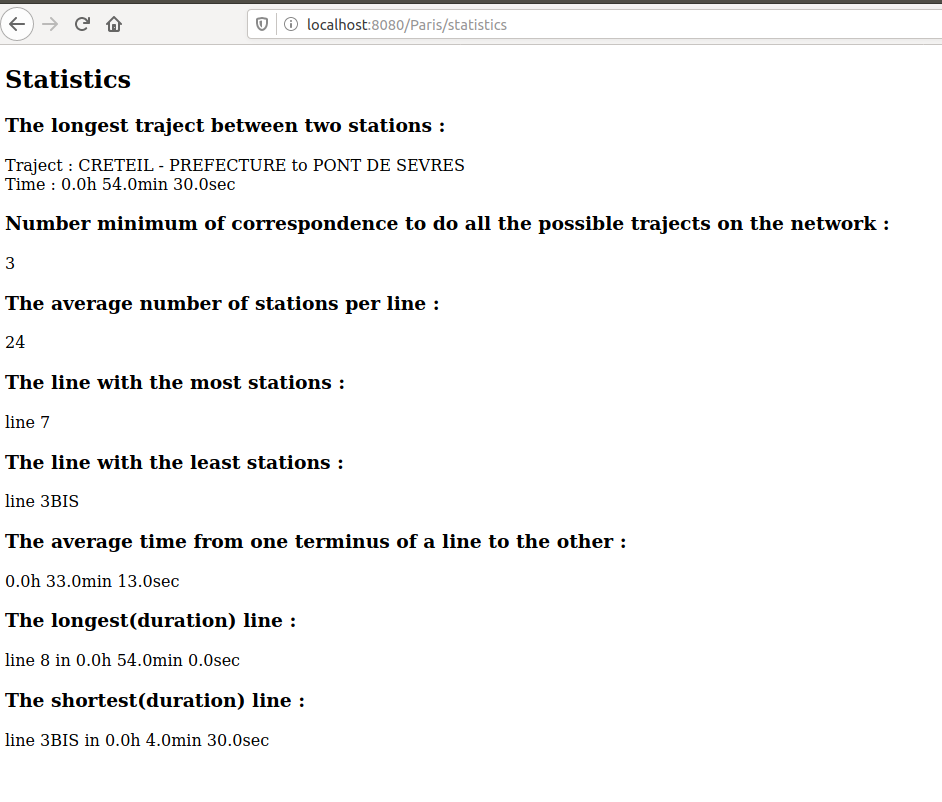
\includegraphics[height=6cm]{images/stat.png}

Voici la fin de cet exemple d'utilisation de "metro" via son webserver.



\newpage

\part{Projet Métro}
Dans cette partie est expliqué les différents algorithmes, la structure des classes du  projet, et sa présentation générale.
\section{Présentation générale}
Voici la présentation du projet avec les choix de modélisation que nous avons fait, les problèmes rencontrés durant celui-ci et la manière dont on l'a organisé.

\subsection{Organisation}
Comme vu précédemment, au début du semestre, nous avons dû faire des choix de modélisation et donc réfléchir. Nous avons d'abord créé le graphe(W\-Graph) car ce graphe représente dans notre réseau de métro.
Parallèlement nous avons créé un parser pour construire un graphe à partir d'un fichier contenant les stations par ligne, d'un réseau de métro.
Nous avons également en un premier temps écrit l'algo de Dijkstra(puis avec la file de priorité).
Nous avons alors pu commencer à écrire les algorithmes avec une limite de correspondances, l'algorithme de Floyd avec les matrices, et l'"algorithme de Bouarah", dont il est parlé dans la section suivante.
Nous avons également ajouter un webserver, car cela commençait à faire lourd de toujours tester sur le terminal.
Nous avons alors rajouté les algorithmes pour les statistiques des réseaux de métro.
Rajoutons que le programme est en anglais car il peut être utilisé pour tout les réseaux de métro. Ici seul ceux en France sont disponible, mais il n'y a pas de problèmes, car il y a juste à stocker le réseau voulu, par un fichier texte adapté, en objet JSON dans les fichiers JSON correspondants.
Nous avons ensuite rajouté la possibilité d'ajouter des perturbations sur nos réseaux métro.
Arrivé à mi-avril, nous avons bien avancé, et il nous reste à améliorer alors notre programme, en rendant un code plus propre et amélioré, améliorer le webserver, régler des bugs, etc...

Notons qu'à chaque tâche attribuée, la personne s'occupant de la tâche doit s'occuper des tests qui vont avec. En général les tâches doivent être faites pour la semaine suivante.
Notre système nous a été efficace, et permis de travailler dans de bonnes conditions.
A chaque fin de tâche, la personne s'en occupant devait attribuer une "merge request" à quelqu'un d'autre pour vérifier son travail et avoir un autre point de vue de la question et voir les éventuels problèmes.
\subsection{Problèmes rencontrés}
Certains problèmes ont été rencontrer durant ce projet.
Au début du projet nous avions le problème de ne pas savoir par où commencer, ou plutôt nous avions peur de partir trop vite en s'emballant ou d'aller trop lentement et perdre du temps. Nous avons donc eu au début du projet, des semaines où il y avait peu de tâches à effectuer et où nous avions du mal à en trouver. Trouver des tâches précises n'était pas non plus facile.
D'où l'importance de s'imprégner vraiment du projet ou d'une partie du projet pour pouvoir décomposer cela en de multiples tâches. Il y a donc eu des tâches trop vagues, et cela a pu être un léger problème par moment. Dans l'implémentation des algorithmes, il y avait ce besoin nécessaire de s'imprégner de l'algorithme pour voir clairement ce que nous voulons. Cela demande un vrai travail de réflexion et de la concentration. Il y a eu une grosse demande de concentration et réflexion pour réussir à faire un bon parser, en cherchant les problèmes qu'il pourrait y avoir dans les modifications que l'on voudrait apporter.
Un autre problème qui peut intervenir et de replonger dans du code que l'on a écrit quelques mois auparavant ou de se plonger dans du code que nous n'avions pas écrit. Le challenge était donc de se maintenir à jour sur les avancées du projet.
Pour les algorithmes, ce qui posait problème, était la réflexion autour de la modélisation pour faire marcher les algorithmes, qui en eux-mêmes n'ont pas posé de problèmes d'implémentations.



\newpage
\section{Les classes plus en détail}
Notre programme a de nombreuses classes de code. On peut y trouver un parser, plusieurs algorithmes, une pour les perturbations, et d'autres pour le webserver. Elles vont être expliquées plus en détail pour le parser et les algorithmes ci-dessous. Nous allons également présenter ci-dessous la structure du projet et de ses classes.
\subsection{Le parser}
Le Parser s'est écrit en plusieurs fois une première version consistait simplement à lire toutes les stations sans faire attention à fourche ou cycle, et crée des doubles liaisons de poids 90 secondes entre une stations, celle écrites auparavant et la suivante. Au moment où cela a été fait sans s'en rendre compte, il n'y avait aucune liaisons qui était créait entre les différentes lignes, elles étaient toutes isolés.\\
C'est la semaine suivante où le Parser fut améliorer et était beaucoup plus fonctionnel. En effet la semaine suivante le parser était retravaillé pour créer des correspondances. Pour ce faire un ensemble des noms de stations déjà créée fût ajouté dans toutes les méthodes du parser et lors de la rencontre d'un nom de station qui est déjà dans cet ensemble on liait cette station (avec un poids de changement de ligne de 60 secondes) avec toutes les autres stations qui avait le même nom (on enlèvera plus tard le cas où le nom de ligne commence par "Meta Station"). \\
Quelque semaine plus tard Dijkstra était implémenter et une première version sur terminal était disponible. Quelque chose nous dérangea dans celle ci, il fallait préciser pour le départ et l'arrivé le nom de la station et la ligne or il parait logique que nous n'ayons qu'à préciser le nom de la station. C'est donc à ce moment que nous avons ajouter des meta stations. Pour chaque station nous avons ajouté une station ayant comme nom de ligne "Meta Station Start" dans laquelle on ne pouvait entrer mais on pouvait aller vers n'importe quelle ligne de la station et une ayant comme ligne "Meta Station End" pour laquelle c'était l'inverse. Toutes ces nouvelles liaisons avait comme poids 0 ce qui faisait qu'elle n'avait aucun poids sur le trajet final. On pouvait désormais lancer les algorithmes de parcours depuis une \emph{meta station start} vers une \emph{meta station end} sans soucis de ligne pour l'utilisateur. \\
Le parser est alors rester comme cela pendant très longtemps, jusqu'à ce que nous nous rendions compte que des changements n'était pas pris en compte lorsque l'on change de branche d'une fourche ou d'un cycle. Il fallu alors ce replonger dans du code qui était assez ancien et cela fût un peu compliqué. Cette partie du parser est celle qui parût la plus compliqué, en effet il fallait séparer les stations qui précéder et suivait un(e) cycle/fourche et modifié les liaisons à celle ci, tout en gérant le cas où ces stations sont liés à d'autre lignes. Au final cela a été fait en sachant qu'il n'existe donc plus de station comme "Botzaris 7bis" (bien qu'il reste ses meta stations), celle ci ayant été remplacé par Botzaris\$1 et Botzaris\$2. Pour éviter d'avoir une multiplications de cas a gérer il se peut que la modélisation du graph ne représente pas dans ce cas la réalité (qui serait que une station \$1 représente un quai et \$2 l'autre). On peut parfois en effet voir dans le cas de fourche que la station \$1 sert par exemple à rentrer dans les fourches tandis que \$2 sert à en sortir. Cela résultera bien dans les temps de parcours cherché, les deux stations étant bien sûr lié d'un poids de changement (= 60).

\subsection{Les différents algorithmes}
Voici une présentation des trois algorithmes de plus court chemin que nous avons utilisé dans ce projet: l'algorithme de Dijkstra, celui de Floyd et celui de Romain Bouarah.
\subsubsection{Dijkstra}
L'algorithme de Dijkstra ne fût pas forcément facile à comprendre. Mais une fois imprégnés de celui-ci, nous avons pu faire un algorithme clair répondant au problème du plus court chemin. Au départ nous n'utilisions pas de file de priorité.
Une fois que l'algorithme marchait, nous avons rajouté les files de priorité en guise d'amélioration.
A partir d'un graphe et d'une station on peut alors lancer l'algorithme avec aussi une hashmap correspondant aux distances des stations par rapport à la station initiale avec le plus court chemin entre elles, et une autre hashmap où chaque clé est une station avec une valeur associée qui est sa station précédente par rapport à la station initiale en prenant le chemin le plus court.
Avant l'analyse du graphe, il y a initialisation de la hashmap en associant des distances à l'infini en valeur pour chaque station(clé) du graphe, et pareil pour la file de priorité.

\subsubsection{Algorithme de Floyd}
Comme dit précédemment, l'algorithme de Floyd a l'avantage d'être relativement simple à comprendre, mais surtout très facile à coder, à condition d'avoir une bonne modélisation d'un graphe sous forme de matrices.
La principale difficulté pour implémenter cet algorithme a donc été la création de ce que nous appellerons des "graphes matrices". Nous avons longtemps hésité entre deux manières de créer de tels graphe: nous avions le choix entre se servir des graphes 
renvoyés par le parser créé pour l'algorithme de Dijsktra, et écrire un nouveau parser que nous utiliserions exclusivement pour l'alogorithme de Floyd. Nous avons opté pour la première option, et le constructeur de la classe MatriceWGraph prend comme arguement, entre autres,
un graphe modélisé par une hashmap. Un graphe matrices est composé de trois matrices: une matrice Direct, où Direct[x][y] = temps de trajet pour aller de la station n'x à la station n'y, une matrice Via, où
Via[x][y] = la dernière station par laquelle on fait un changement pour aller de la station n'x à la station n'y (si il n'ya pas de changement à faire, Via[x][y] = station n'x), et enfin une matrice Intermediate, où
Intermediate[x][y] = nombre de correspondance pour aller de la station n'x à la station n'y (si les deux stations sont sur la même ligne, on a tout simplement Intermediate[x][y] = 1$, et $Intermediate[x][x] = 0).
Seuls les coefficients correspondant faisant le lien entre deux stations sur la même ligne sont au départ initialisés. Ces l'algorithme de Floyd, que nous lançons sur ces trois matrices, qui nous permet de remplir tous les coefficients.  

\subsubsection{Algorithme de Romain Bouarah}
L'algorithme de Romain Bouarah est une alternative à l'algorithme de Floyd pour trouver des chemins en un nombre limité de correspondances.

\paragraph{Origine}
Cet algorithme est une réponse au besoin pressant d'obtenir des chemins avec un minimum de correspondances.
En effet, l'implémentation de l'algorithme de Floyd était difficile et ça faisait presque 3 semaines que nous travaillions dessus avec ardeur.
La construction du graphe sous forme de matrice posait problème notamment les cycles, fourches et stations partagées par plusieurs lignes.
C'est pour cela que cet algorithme a été imaginé.

\paragraph{Difficultés}
Bien que cet algorithme travaille directement sur le graphe, il y a, hélas, encore quelques cas à prendre en compte :

\begin{quote}  
  La principale difficulté était de faire cohabiter des chemins courts avec un nombre de correspondances élevé avec des mêmes chemins plus long mais avec moins de correspondances, en effet il était impossible de garder qu'un seul type de chemin au risque d'élaguer une grande partie de l'arbre d'exploration.
\end{quote}

\paragraph{Solution}
La solution fut alors de multiplier le graphe par un nombre maximal de correspondances, en faisant cela des noeuds atteints avec un nombre de correspondances différents pouvaient exister ensemble.
Au final, le groupe était redevenu optimiste car nous avions échappé à la ``tempête Floyd''.

\newpage
\subsection{Structure des classes}
%Diagramme des classes à rajouter
Voici donc la version du diagramme uml des classes du projet, on peut également le trouver sur le projet dans le dossier dossier doc/diagram. Il y a donc les classes WGraph et Parser qui permmettent la construction de graphes à partir de fichiers textes. Les classes Dijkstra(PriorityQueue est utilisé dedans), BouarahAlgorithm, MatriceWgraph, LimitedConnectionResearch qui sont les classes des algorithmes de recherches de plus court chemin. Il y a la classe Trafics pour ajouter des perturbations, Initialize pour l'exécution sur terminal, App pour qui a un seul main appelé lors de l'exécution sur terminal. Statistics est la classe où sont regroupés tout les algorithmes de statistiques. Il y a la classe Configuration pour les villes avec un réseau de métro, GraphExporter pour se représenter visuellement le graphe. La classe Station elle, représente l'objet station, avec un nom de station et une ligne associée.


\rotatebox{90}{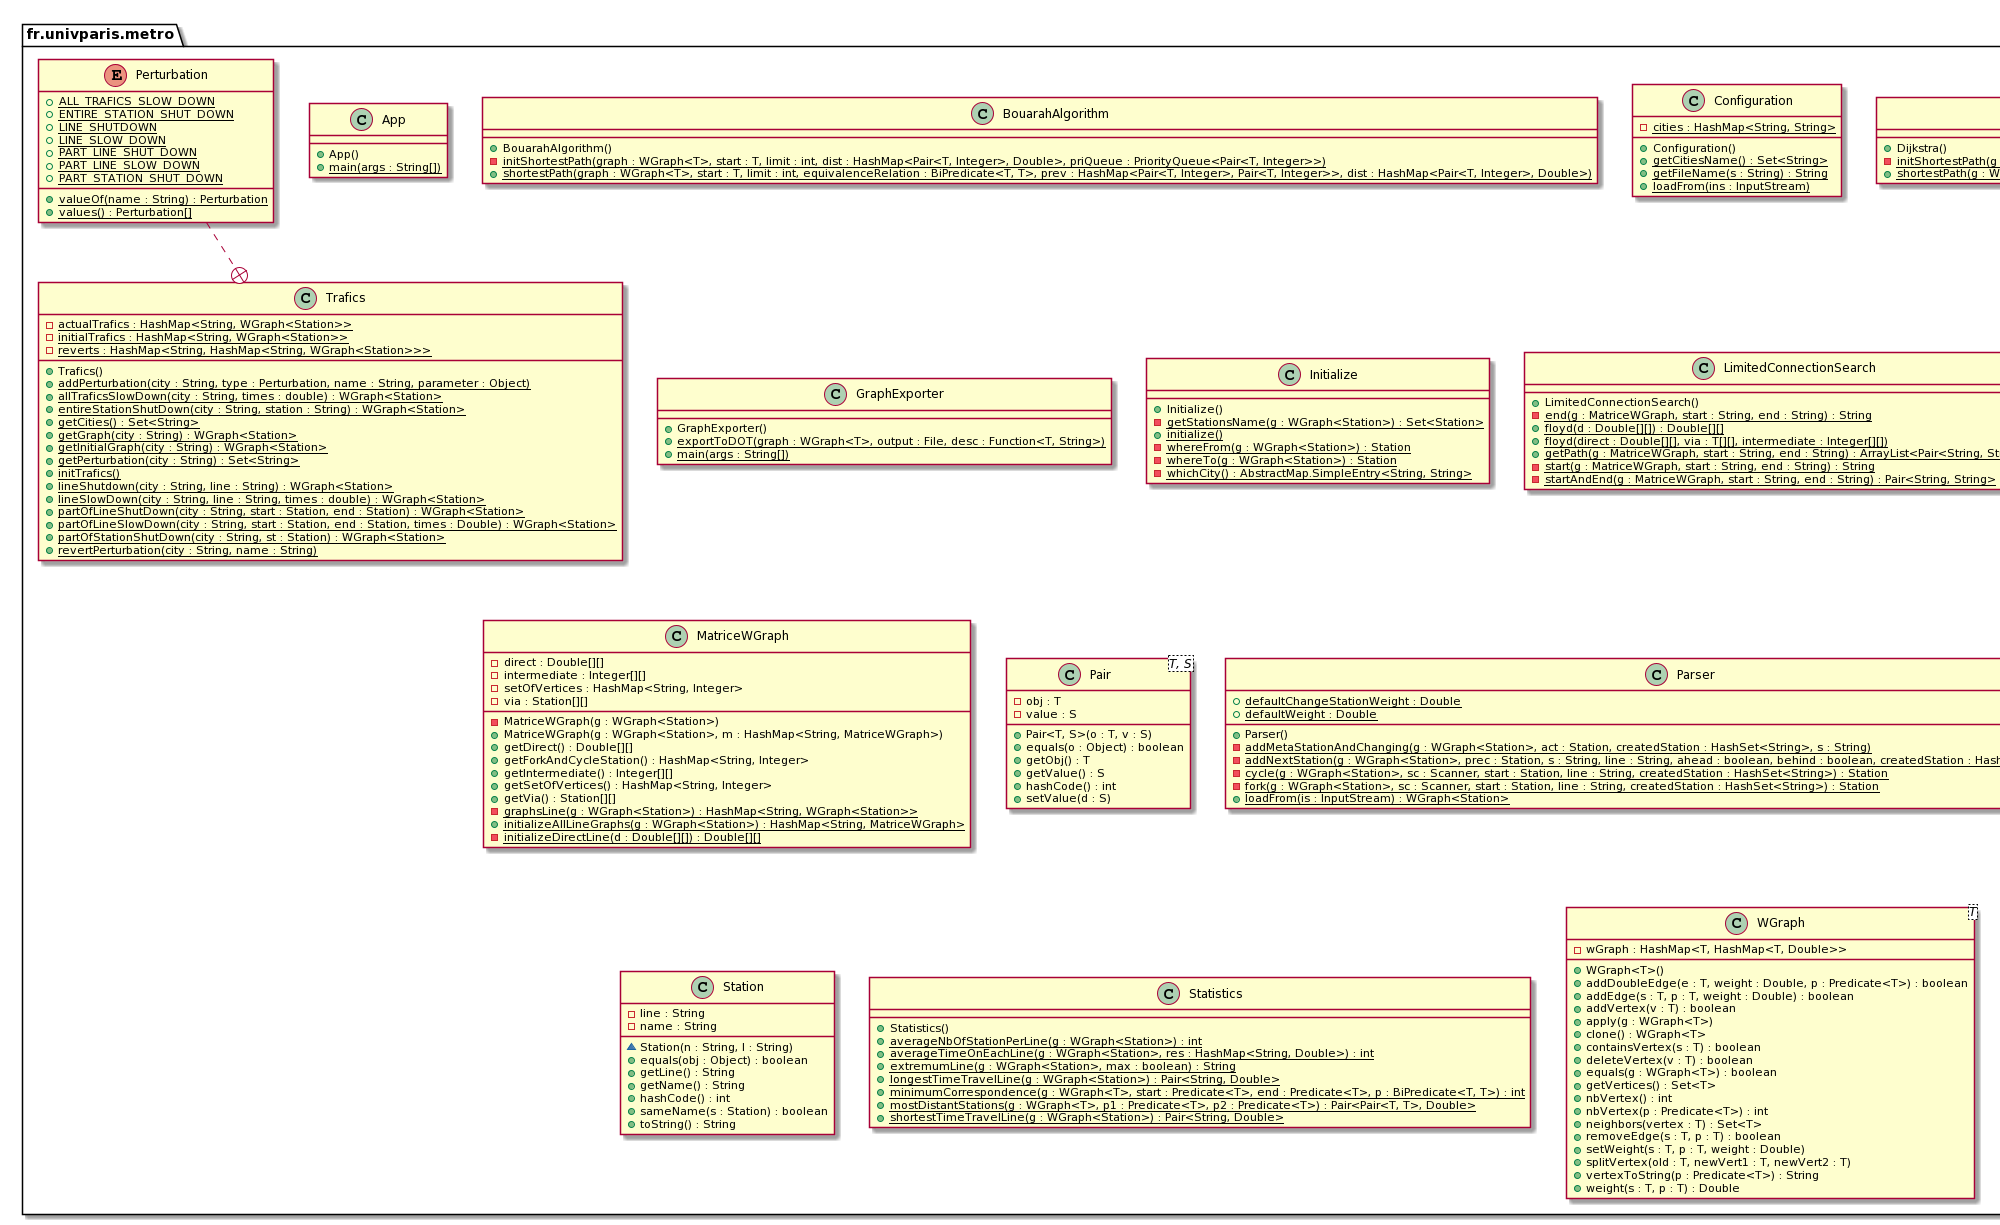
\includegraphics[width=20cm]{images/diagram08052020}}

\end{document}
